\documentclass[a4paper]{article}
\usepackage[margin=1in]{geometry}
\usepackage{ctex}
\usepackage{lipsum}
\usepackage{longtable}
\usepackage{graphicx}
\usepackage{caption}
\captionsetup[figure]{font = small}

\title{铅酸电池放电时间预测}
\author{许博涵 \and 申思远}
\begin{document}
\maketitle

\section{问题一}\label{sec:big-title}

\paragraph{首先我们使用$readmatrix()$读取data.xlsx文件中附件一的数据,并进行数据有效性处理。}

\subsection{问题分析}
通过观察数据散点图,可以先假设模型,决定采用什么样的拟合函数,再使用$polyfit()$或$fittype()$函数进行图像拟合,进而求出放电函数曲线。通过筛选出从$U_m$开始按不超过$0.005V$的最大间隔的231个样本点,记录其对应的电压和已放电时间$T_r$利用上一步求出的拟合函数计算出估计放电时间$T_p$,通过公式
\begin{equation}\label{eq1}MRE = \frac{{|{T_p} - {T_r}|}}{{{T_r}}}\end{equation}
可以计算出相对误差,分别求出231个样本点的相对误差,再求出平均值即可得到平均相对误差。最后一问,直接将$9.8V$这个数据带入拟合函数即可。
\subsection{模型假设}
我们使用MATLAB软件,我们以时间为电压,绘制出已放电时间$T$与电压$U$的关系图像,如图1所示。
\begin{figure}[htbp]
    \centering
    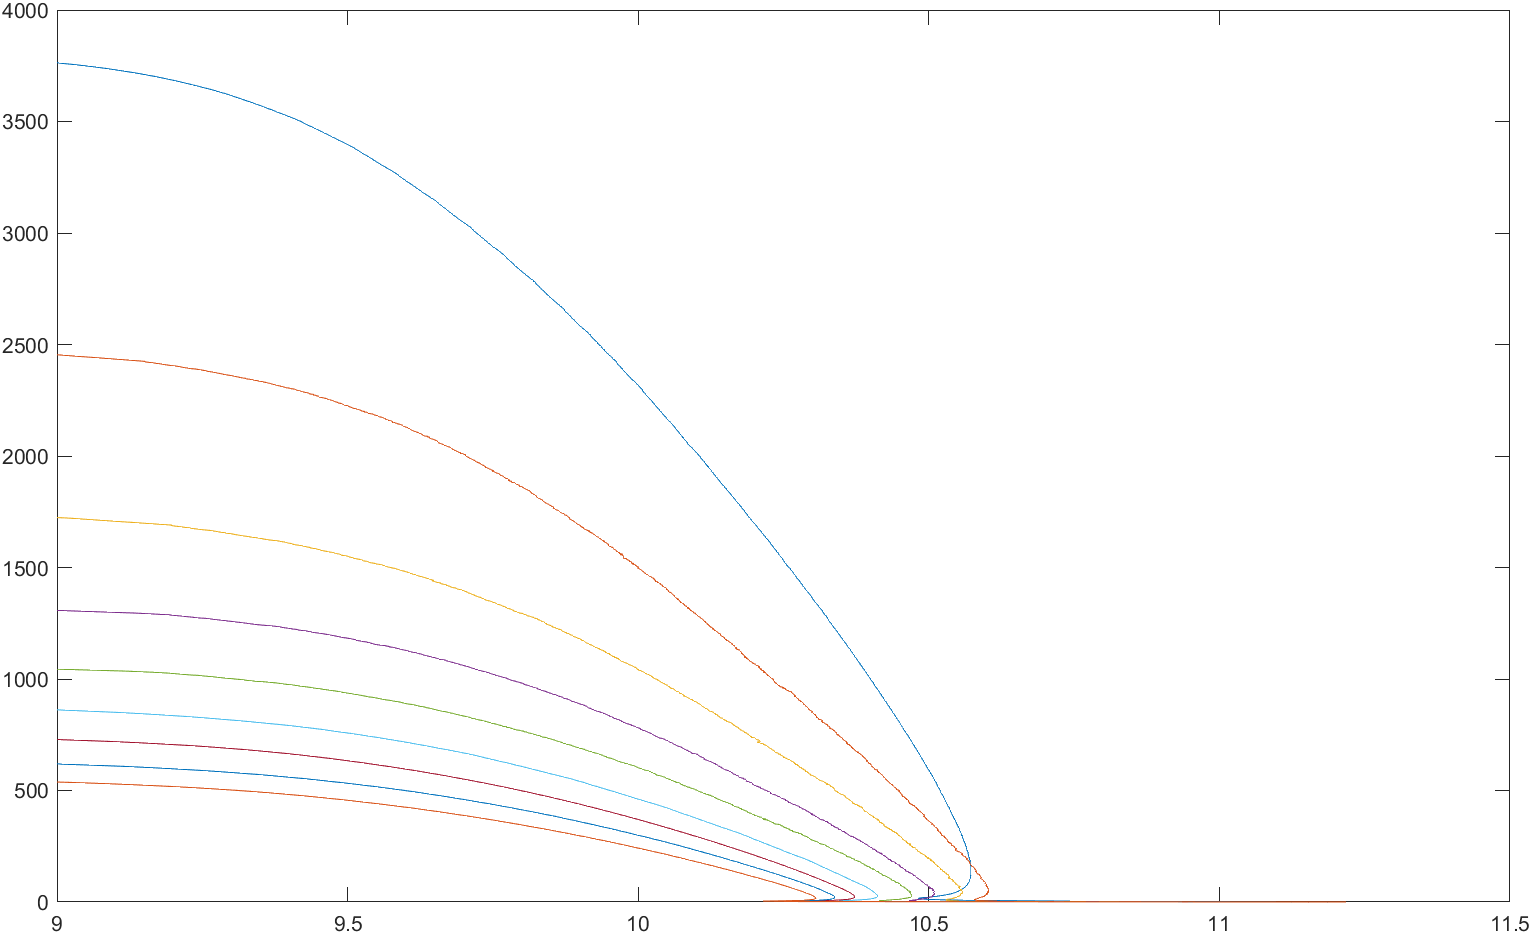
\includegraphics[width = 0.6\textwidth]{img/1.png}
    \caption{电压与已放电时间的关系}
\end{figure}

由图一可知,不同电流强度随放电时间的变化趋势基本一致,初步假设采用5次多项式进行拟合。
\subsection{符号说明}
\begin{table}[htbp]
    \begin{center}
        \setlength\tabcolsep{40pt}
        \renewcommand{\arraystretch}{1.4}
        \begin{tabular}{c c}
            \hline
            符号    & 含义     \\ \hline
            $U_m$ & 最低保护电压 \\
            $T_r$ & 样本时间   \\
            $T_p$ & 预测时间   \\
            $T$   & 已放电时间  \\
            $U$   & 电压     \\
            $I$   & 电流     \\
            $MRE$ & 平均相对误差 \\
            \hline
        \end{tabular}
    \end{center}
\end{table}
\subsection{模型建立}
但是我们注意到,在电流$I$时,刚开始放电初期电压不稳定,对于模型的建立和拟合都会造成影响,故我们在进行拟合时剔除了前$20\%$的数据。根据图1决定采用了5次多项式进行拟合。
\subsection{模型求解}
我们使用MATLAB软件中的$polyfit()$函数直接进行拟合出5次多项式。结果如图2所示。
\begin{figure}[htbp]
    \centering
    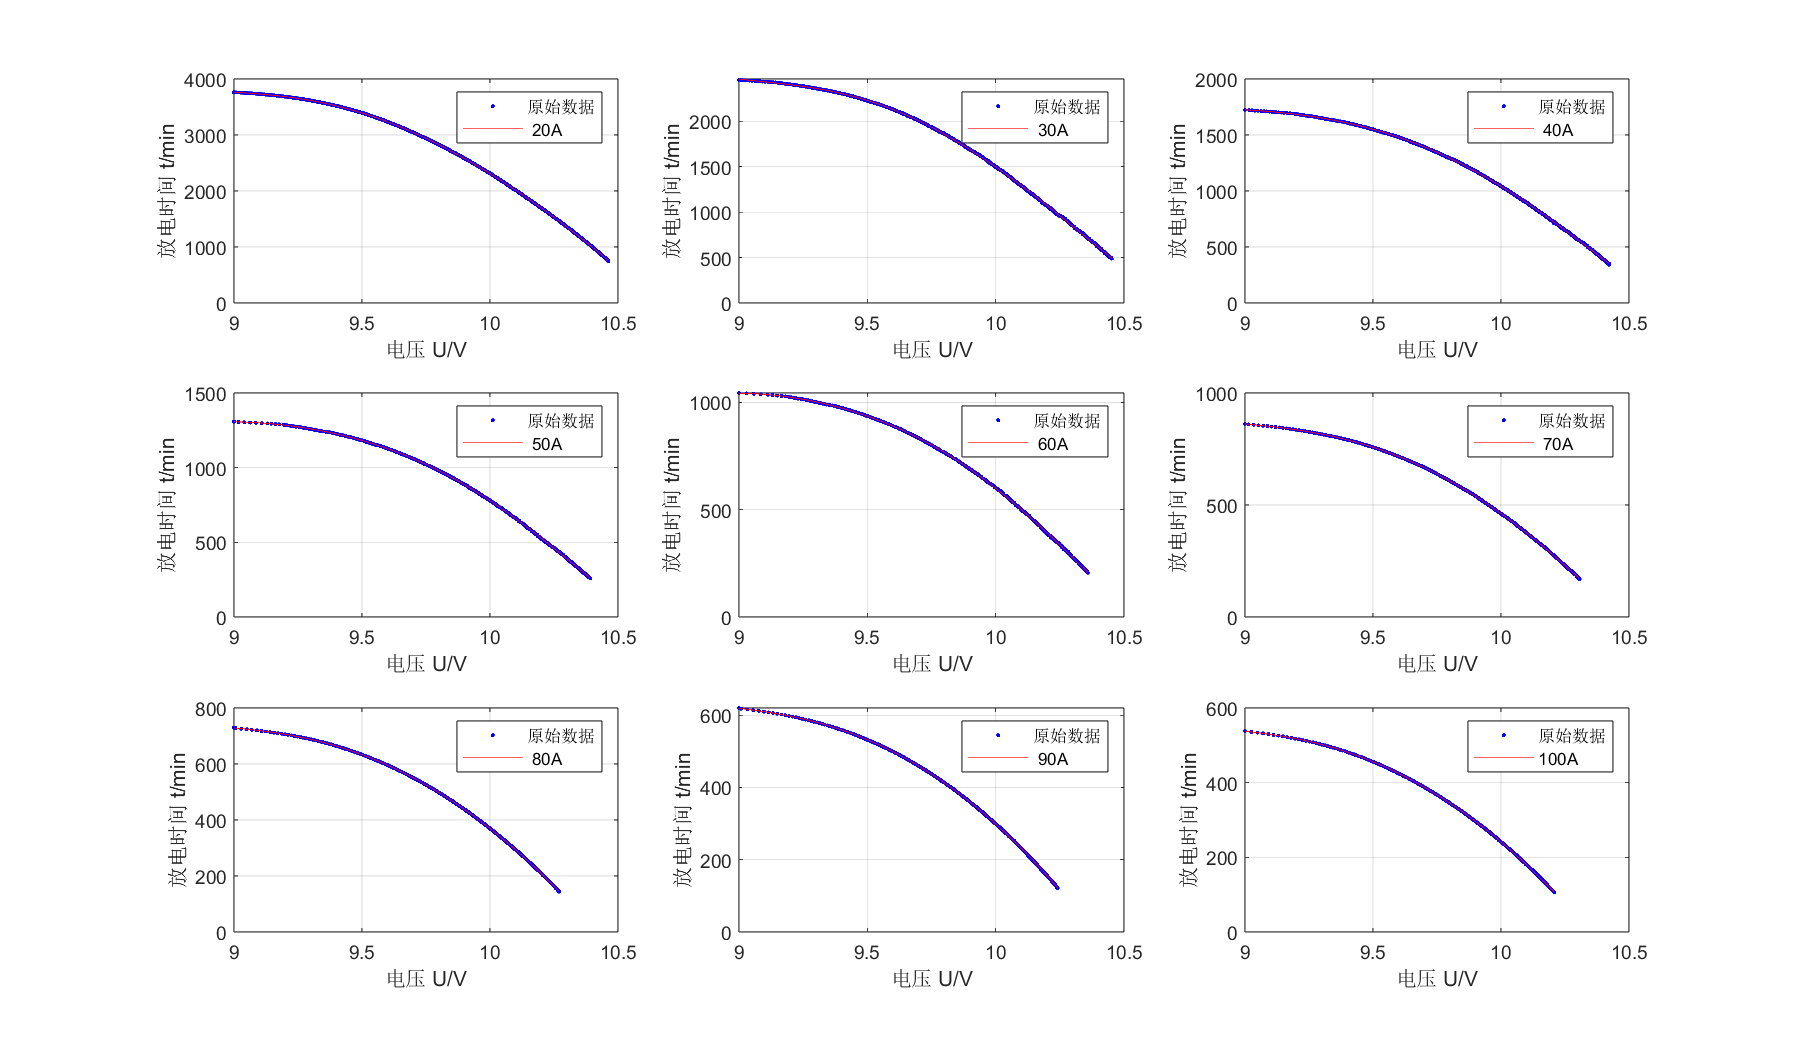
\includegraphics[width = 1.0\textwidth]{img/2.png}
    \caption{各电流状态下的拟合图像}
\end{figure}
\subsection{结果分析}
我们首先计算出各个相邻点的差值,然后筛选出231个差值小于0.005的点,记录这些点的已放电时间$T_r$和电压值,再将电压值代入拟合函数求出$T_p$。接着利用公式(1)求出每个电流对应的平均相对误差$MRE$如下表1:
\begin{table}[htbp]
    \centering
    \begin{center}
        \begin{tabular}{|c|c|c|c|c|c|c|c|c|c|}
            \hline
            电流    & 20A     & 30A     & 40A     & 50A     & 60A     & 70A     & 80A     & 90A     & 100A     \\ \hline
            $MRE$ & 0.022\% & 0.076\% & 0.122\% & 0.092\% & 0.146\% & 0.137\% & 0.073\% & 5.697\% & 13.799\% \\ \hline
        \end{tabular}
        \caption{各个电流状态下对应的$MRE$}
        \label{tab:my-table}
    \end{center}
\end{table}

总体来说求出的平均相对误差$MRE$都较小,说明采用5次多项式拟合可行。

\section{问题二}
\subsection{问题分析}
可以判定,不同电流强度下的放电曲线之间正相关,即它们可以用相似的表达式表示;结合$U(I,T)=a(T_{max}(I)-T)^b+9$可知,将表达式的系数看作是电流强度$I$的函数,我们建立电压与电流强度、时间的二元抛物线模型。
\subsection{模型假设}
电压与电流强度、时间的二元抛物线模型$U(I,T)=a(I)(T_{max}(I)-T)^b(I)+9$。
\subsection{模型建立}
我们使用MATLAB软件中的$polyfit()$函数直接进行拟合。对比寻找最优的n次多项式。
\subsection{符号说明}
\begin{table}[htbp]
    \begin{center}
        \setlength\tabcolsep{40pt}
        \renewcommand{\arraystretch}{1.4}
        \begin{tabular}{c c}
            \hline
            符号        & 含义      \\ \hline
            $a(I)$    & 电流强度$I$ \\
            $b(I)$    & 电流强度$I$ \\
            $Tmax(I)$ & 电流强度$I$ \\
            \hline
        \end{tabular}
    \end{center}
\end{table}
\subsection{模型建立}
利用附件1,我们查找出9种电流强度下的电池最大放电时间
\begin{table}[htbp]
    \centering
    \begin{center}
        \begin{tabular}{|c|c|c|c|c|c|c|c|c|c|}
            \hline
            电流        & 20A  & 30A  & 40A  & 50A  & 60A  & 70A & 80A & 90A & 100A \\ \hline
            $T_{max}$ & 3764 & 2454 & 1724 & 1308 & 1044 & 862 & 730 & 620 & 538  \\ \hline
        \end{tabular}
        \caption{9种电流强度下的电池最大放电时间}
        \label{tab:my-table}
    \end{center}
\end{table}
\begin{table}[htbp]
    \centering
    \begin{center}
        \begin{tabular}{|c|c|c|c|c|c|c|c|c|c|}
            \hline
            电流        & 20A  & 30A  & 40A  & 50A  & 60A  & 70A & 80A & 90A & 100A \\ \hline
            a  & 0.024 & 0.312 & 0.037 & 0.049 & 0.052 & 0.048 & 0.048 & 0.049 & 0.049 \\ \hline
            b  & 0.514 & 0.505 & 0.504 & 0.481 & 0.484 & 0.505 & 0.515 & 0.521 & 0.530 \\ \hline    
        \end{tabular}
        \caption{不同电流强度下的方程系数}
        \label{tab:my-table}
    \end{center}
\end{table}

\subsection{模型求解}
我们使用 MATLAB 软件中的$polyfit()$函数直接进行拟合。对比寻找最优的$n$次多项式。
\begin{figure}[htbp]
    \centering
    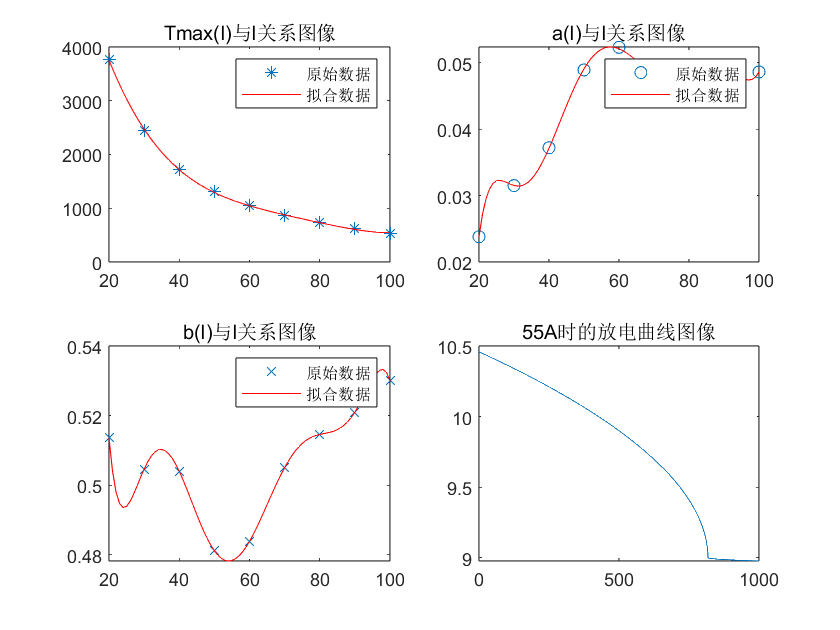
\includegraphics[width = 1.0\textwidth]{img/4.png}
\end{figure}
\end{document}